\documentclass[10pt, compress]{beamer}

\usetheme[numbering=fraction, progressbar=none, titleformat=smallcaps, sectionpage=none]{metropolis}
\usepackage{booktabs}
\usepackage{array}
\usepackage{listings}
\usepackage{graphicx}
\usepackage[english]{babel}
\usepackage[scale=2]{ccicons}
\usepackage{url}
\usepackage{relsize}
\usepackage{wasysym}

\usepackage{pgfplots}
\usepgfplotslibrary{dateplot}

\lstset{ %
  backgroundcolor={},
  basicstyle=\ttfamily\footnotesize,
  breakatwhitespace=true,
  breaklines=true,
  captionpos=n,
  commentstyle=\color{orange},
  escapeinside={\%*}{*)},
  extendedchars=true,
  frame=n,
  keywordstyle=\color{orange},
  language=C++,
  rulecolor=\color{black},
  showspaces=false,
  showstringspaces=false,
  showtabs=false,
  stepnumber=2,
  stringstyle=\color{gray},
  tabsize=2,
  keywords={thrust,plus,device_vector, copy,transform,begin,end, copyin,
  copyout, acc, \_\_global\_\_, void, int, float, main, threadIdx, blockIdx,
  blockDim, if, else, malloc, NULL, cudaMalloc, cudaMemcpy, cudaSuccess,
  cudaGetLastError, cudaDeviceSynchronize, cudaFree, cudaMemcpyDeviceToHost,
  cudaMemcpyHostToDevice, const, data, independent, kernels, loop,
  fprintf, stderr, cudaGetErrorString, EXIT_FAILURE, for, dim3},
  otherkeywords={::, \#pragma, \#include, <<<,>>>, \&, \*, +, -, /, [, ], >, <}
}

\renewcommand*{\UrlFont}{\ttfamily\smaller\relax}

\graphicspath{{../img/}}

\title{Introduction to GPU Programming \\ with the CUDA Platform}
\author{\footnotesize Pedro Bruel \\ {\scriptsize phrb@ime.usp.br}}
\institute{
\includegraphics[height=2cm]{imelogo}\\[0.2cm] Instituto de Matemática e Estatística \\ Universidade de São Paulo}
\date{\scriptsize 4th INFIERI, 2017}

\begin{document}

\part{Part I}

\maketitle

\section{Introduction}

\subsection{About}

\begin{frame}
    \frametitle{About}
    \footnotesize
    \begin{columns}[T,onlytextwidth]
        \column{0.5\textwidth}
        \begin{center}
            \includegraphics[width=.42\textwidth]{pedro}

            Pedro Bruel

            \alert{phrb}@ime.usp.br
        \end{center}

        \column{0.5\textwidth}
        \begin{center}
            \includegraphics[width=.37\textwidth]{alfredo}

            Alfredo Goldman

            \alert{gold}@ime.usp.br
        \end{center}

    \end{columns}

    \begin{center}
        \includegraphics[width=.18\textwidth]{gubi}

        Marco Dimas Gubitoso

        \alert{gubi}@ime.usp.br
    \end{center}
\end{frame}

\subsection{Summary}

\begin{frame}
    \frametitle{Part I}
    \setbeamertemplate{section in toc}[sections numbered]
    \tableofcontents[hideallsubsections, part=1]
\end{frame}

\begin{frame}
    \frametitle{Part II}
    \setbeamertemplate{section in toc}[sections numbered]
    \tableofcontents[hideallsubsections, part=2]
\end{frame}

\begin{frame}
    \frametitle{Slides}
    \begin{center}
        \includegraphics[width=.18\textwidth]{github}
    \end{center}
    This presentation and all source code are available
    at \alert{GitHub}:

    \begin{itemize}
        \item \url{github.com/phrb/intro-cuda}
    \end{itemize}
\end{frame}

\section{Heterogeneous Computing}

\subsection{Hardware Acceleration}

\begin{frame}
    \frametitle{Hardware Acceleration}
    \begin{center}
        \includegraphics[width=.6\textwidth]{accelerate}
    \end{center}

    The use of \alert{devices} to accelerate computations on large datasets:
    \pause
    \begin{itemize}
        \item Associated with a \alert{host} processor
            \pause
        \item Separate \alert{control} and \alert{memory}
            \pause
        \item Differ on \alert{specialization} and \alert{configurability}
            \pause
        \item \alert{GPUs}, DSPs, FPGAs, ASICs
    \end{itemize}
\end{frame}

\begin{frame}
    \frametitle{Hardware Acceleration}
    Use cases:
    \begin{itemize}
        \item Machine Learning
        \item Digital Signal Processing
        \item Bioinformatics
        \item Cryptography
        \item Meteorology
        \item Simulations
        \item ...
    \end{itemize}
\end{frame}

\begin{frame}
    \frametitle{Hardware Acceleration}
    \centering
    \includegraphics[width=.8\textwidth]{accel}
\end{frame}

\begin{frame}
    \frametitle{Hardware Acceleration}
    Percentage of systems with accelerators in the \textit{Top500}:

    \begin{center}
    \includegraphics[width=.95\textwidth]{top500_accel}
    \hfill

        \tiny{Image: \url{top500.org/lists/2016/06/download/TOP500_201606_Poster.pdf} [Accessed in 29/07/16]}
    \end{center}
\end{frame}

\subsection{Heterogeneous Computing}

\begin{frame}
    \frametitle{Heterogeneous Computing}
    \begin{center}
        \includegraphics[width=.83\textwidth]{titan}
    \end{center}

    \pause

    Given \alert{heterogeneous} computational resources, \alert{datasets}
    and a set of \alert{computations}, how to distribute data and computations
    to \alert{optimize resource usage}?
    \hfill

    \begin{center}
    \tiny{Image: \url{olcf.ornl.gov/titan} [Accessed in 29/07/16]}
    \end{center}
\end{frame}

\begin{frame}
    \frametitle{Heterogeneous Computing}
    \alert{Heterogeneous} computational resources:
    \pause
    \begin{itemize}
        \item Low latency: CPUs
            \pause
        \item High Throughput: GPUs
            \pause
        \item Reconfigurable: FPGAs
            \pause
        \item Specialized: ASICs, DSPs
            \pause
        \item Memory?
    \end{itemize}
\end{frame}

\begin{frame}
    \frametitle{Heterogeneous Computing}
    \alert{Datasets}:
    \begin{itemize}
        \item \textit{Big Data}
        \item \textit{Data Streams}
        \item ...
    \end{itemize}
    \pause
    Programming models (\alert{computations}):
    \begin{itemize}
        \item \textit{MapReduce}
        \item \textit{Task Parallelism}
        \item ...
    \end{itemize}
\end{frame}

\begin{frame}
    \frametitle{Heterogeneous Computing: Scalability}
    \begin{center}
        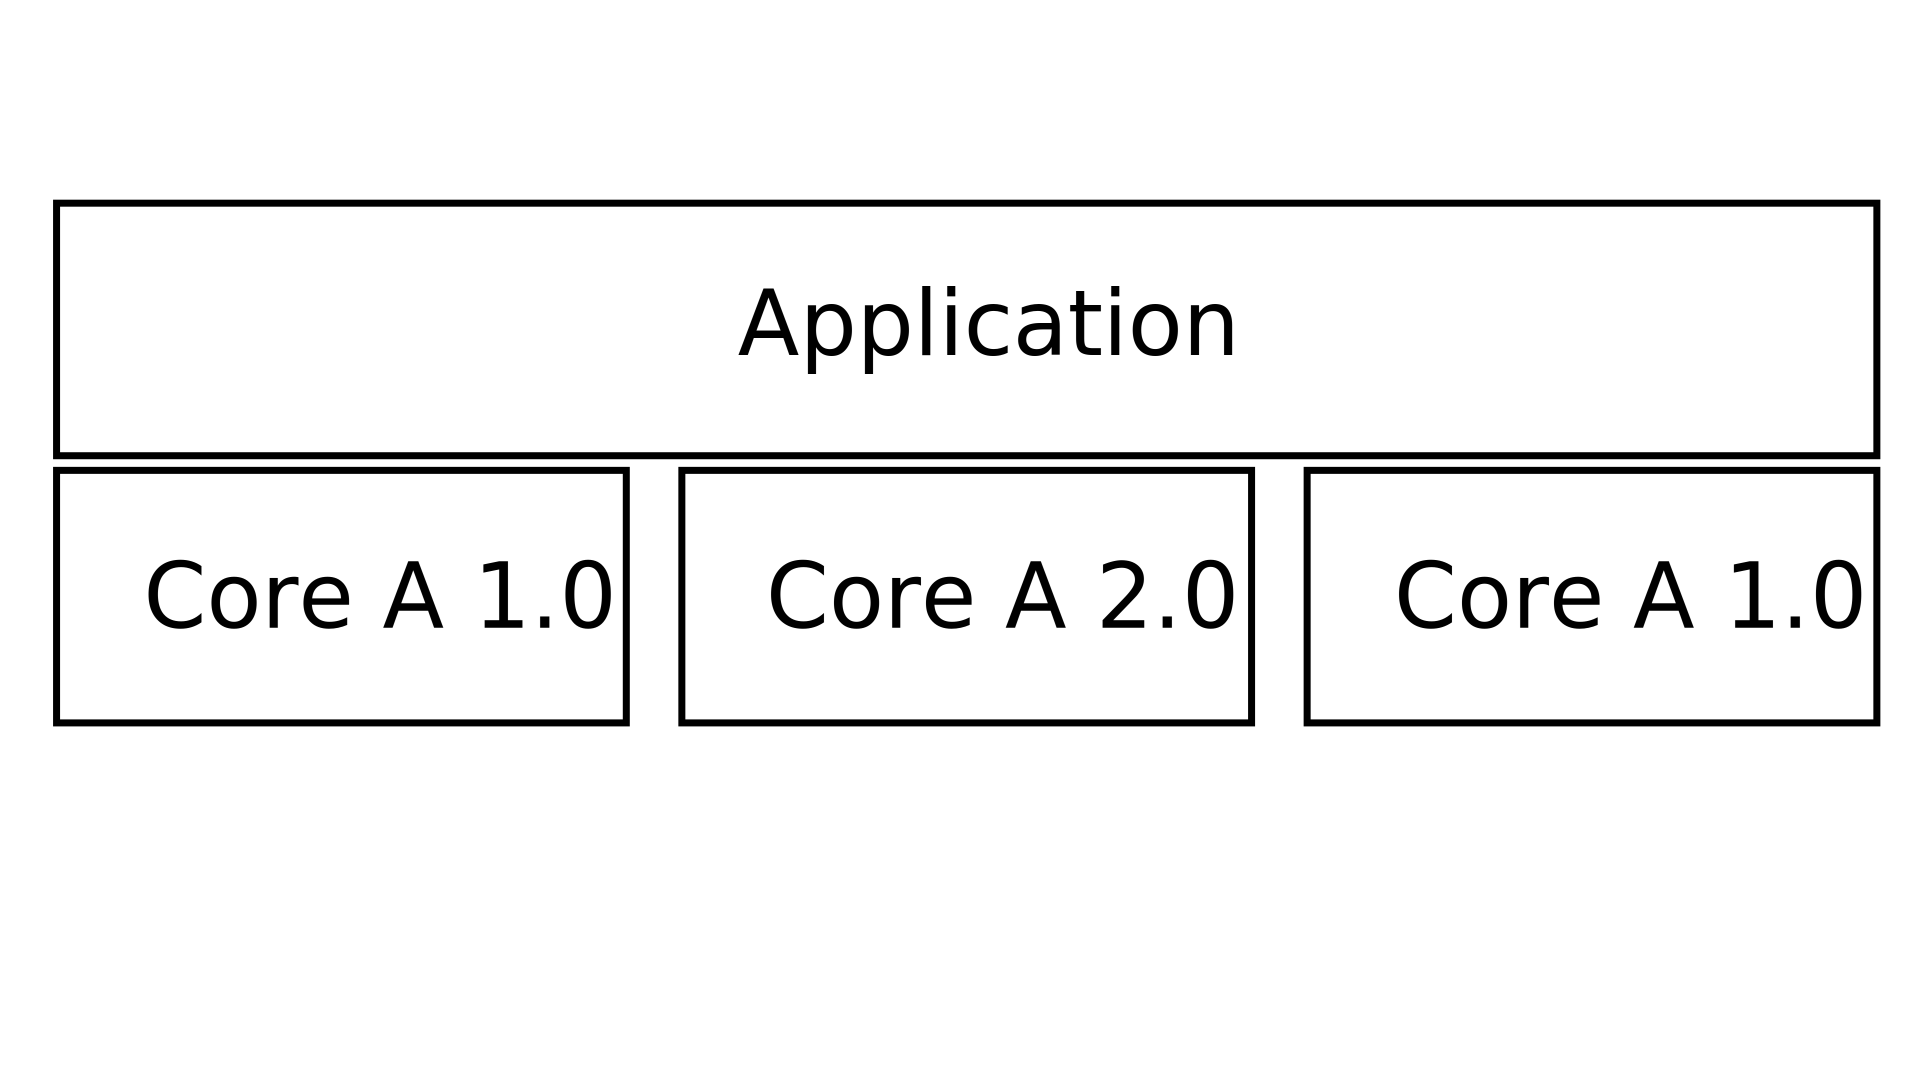
\includegraphics[width=.7\textwidth]{scalability}
    \end{center}

    \alert{Scalability} means not losing performance running in:
    \begin{itemize}
        \item Multiple identical cores
            \pause
        \item New versions of the same core
    \end{itemize}
\end{frame}

\begin{frame}
    \frametitle{Heterogeneous Computing: Portability}
    \begin{center}
        \includegraphics[width=.7\textwidth]{portability}
    \end{center}

    \alert{Portability} means not losing performance running in different:
    \begin{itemize}
        \item Cores or \alert{accelerators}
            \pause
        \item Memory models
            \pause
        \item Parallelism models
            \pause
        \item Instruction sets
    \end{itemize}
\end{frame}

\begin{frame}
    \frametitle{Heterogeneous Computing}
    \centering
    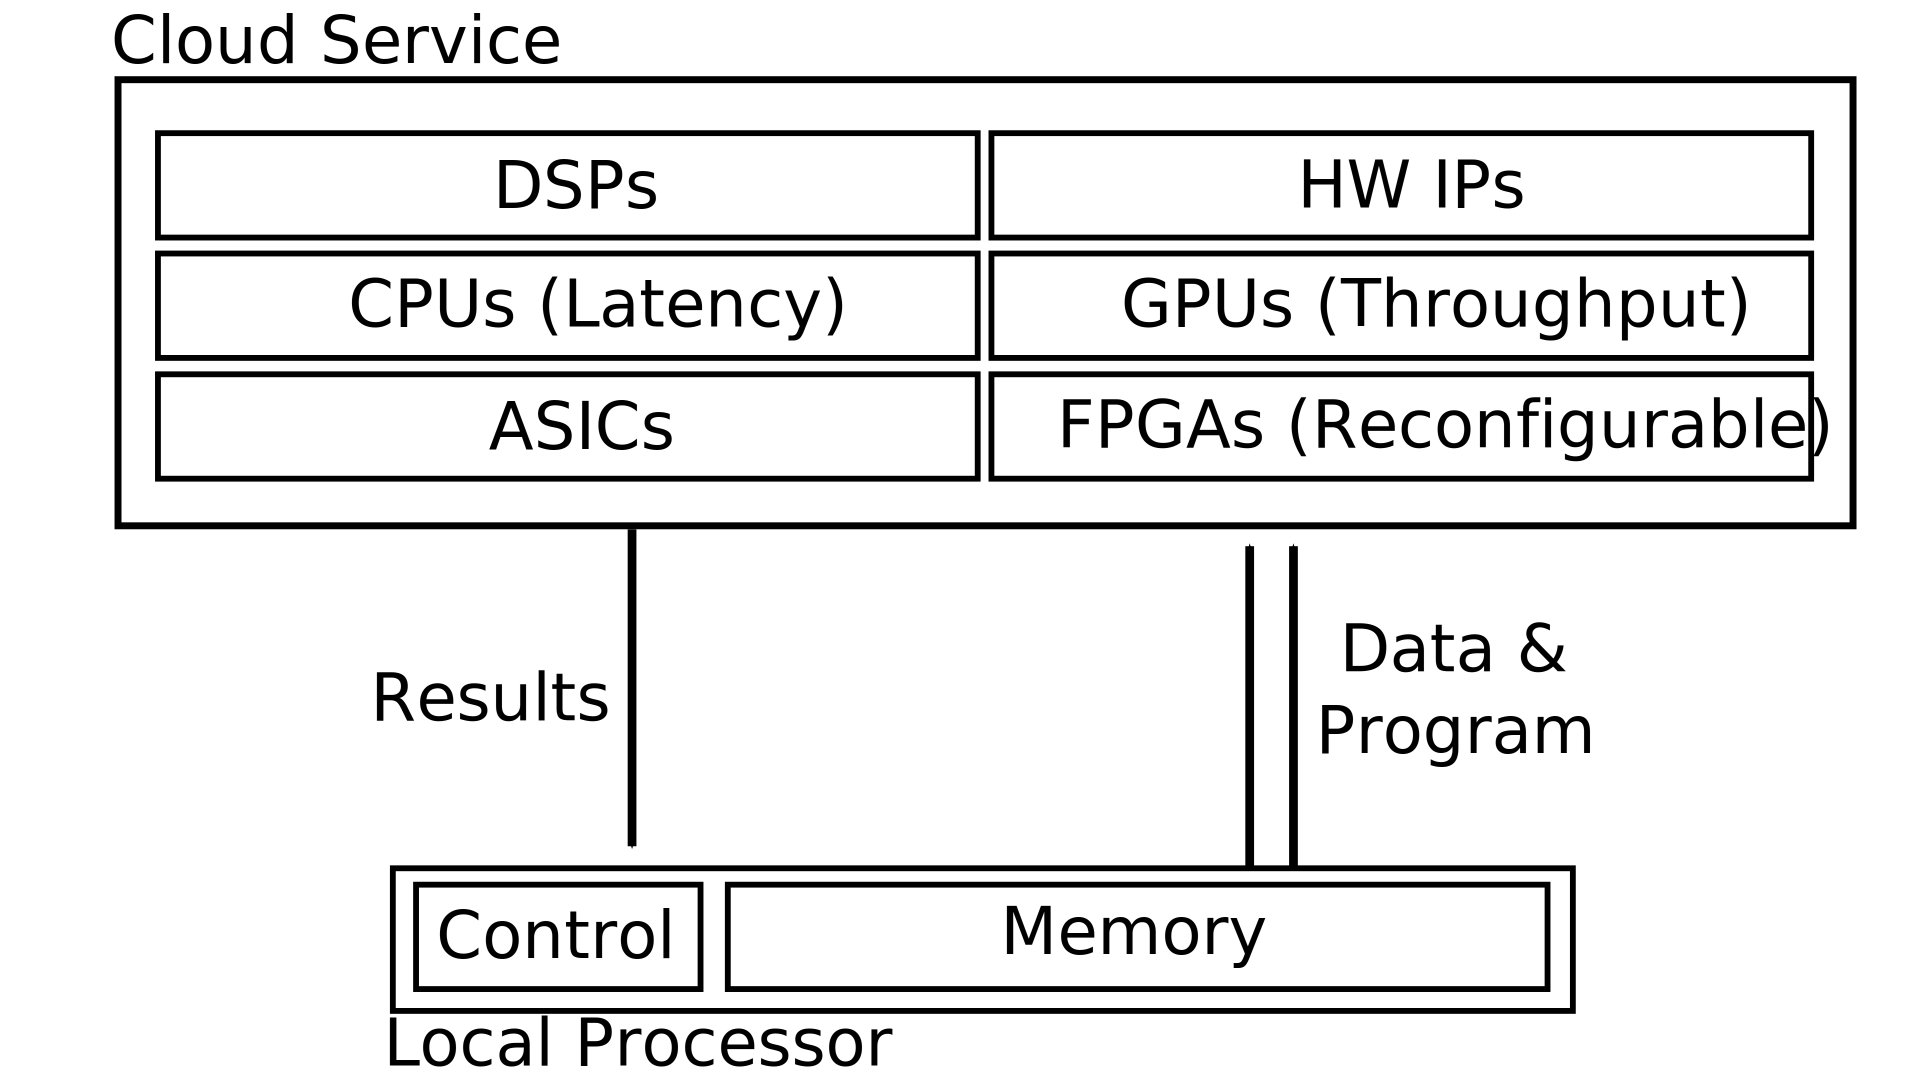
\includegraphics[width=.85\textwidth]{heterogeneous}
\end{frame}

\begin{frame}
    \frametitle{Heterogeneous Computing}
    \centering
    \includegraphics[width=.85\textwidth]{heterogeneous_highlight}
\end{frame}

\section{GPUs}

\begin{frame}
    \frametitle{Graphics Processing Units}
    \begin{center}
        \includegraphics[width=.6\textwidth]{gtx1080}
    \end{center}
    \pause

    Originally specialized for \alert{graphical processing},
    optimized for large datasets and \alert{high throughput}:
    \pause

    \begin{itemize}
        \item Small caches (\textit{kilobytes})
            \pause
        \item No \alert{branch prediction}
            \pause
        \item Thousands of \alert{higher latency} ALUs
            \pause
        \item Execution \alert{pipelines}
            \pause
        \item 114 688 concurrent \alert{threads} in Pascal architecture
    \end{itemize}
\end{frame}

\begin{frame}
    \frametitle{Graphics Processing Units}
    Now, largely used in general-purpose computing,
    also called \textit{General Purpose GPUs} (GPGPUs):
    \pause
    \begin{itemize}
        \item \textit{OpenGL}: 1992
        \item \textit{DirectX}: 1995
        \item \alert{CUDA}: 2007
        \item \textit{OpenCL}: 2009
        \item \textit{Vulkan}: 2016
    \end{itemize}
\end{frame}

\subsection{Hardware Model}

\begin{frame}
    \frametitle{Hardware Model}
    Flynn's taxonomy:
    \begin{itemize}
        \item \textit{Single Instruction Multiple Data} (SIMD)
            \pause
        \item \textit{Single Instruction Multiple Thread} (SIMT)?
    \end{itemize}
    \pause
    Scheduling and execution:
    \begin{itemize}
        \item \textit{Streaming Multiprocessor} (SM)
            \pause
        \item \textit{Warps}
            \pause
        \item \textit{Grids, blocks} and \textit{threads}
    \end{itemize}
\end{frame}

\begin{frame}
    \frametitle{Hardware Model}
    Higher-Level scheduling:
    \begin{itemize}
        \item \textit{Pipelines}
        \item \textit{Texture Processing Cluster} (TPC)
        \item \textit{Graphics Processing Cluster} (GPC)
    \end{itemize}
    \pause
    Memory:
    \begin{itemize}
        \item Shared: L1, L2 caches; \textit{megabytes} (NVIDIA Pascal)
        \item Global: volatile, GDDR5; \textit{gigabytes}
            \pause
        \item SSD: \alert{non-volatile}; \alert{\textit{terabytes}} (AMD SSG Fiji, 2017)
    \end{itemize}
    \vfill

    \tiny{AMD SSG: \url{anandtech.com/show/10518/amd-announces-radeon-pro-ssg-fiji-with-m2-ssds-onboard} [Accessed in 30/07/16]}
\end{frame}

\subsection{Compute Capability and SIMT}

\begin{frame}
    \frametitle{\textit{Compute Capability} and SIMT}
    The \alert{Compute Capability} specifies \textit{Single Instruction
    Multiple Thread} (SIMT) architectures:
    \pause
    \begin{itemize}
        \item \textit{Warp}: Group of \textit{threads} that runs in \alert{parallel}
        \item \textit{Streaming Multiprocessor} (SM): Creates, schedules and runs \textit{warps}
            \pause
        \item Multiple \textit{warps} run \alert{concurrently} in a SM
    \end{itemize}
    \vfill

    \begin{center}
        \tiny{Source: \url{docs.nvidia.com/cuda/cuda-c-programming-guide/index.html\#hardware-implementation} [Accessed in 29/07/16]}
    \end{center}
\end{frame}

\begin{frame}
    \frametitle{\textit{Compute Capability} and SIMT}
    \textit{Warps}:
    \pause
    \begin{itemize}
        \item Unit of execution and scheduling
        \item 32 \textit{threads}
            \pause
        \item 1 \alert{common instruction} at a time
            \pause
        \item \textit{Active threads}: in the current execution branch
        \item \textit{Inactive threads}: \alert{not} in the current execution branch
            \pause
        \item Inactive threads run \alert{sequentially}
            \pause
        \item Efficiency: no execution divergence inside \textit{Warps}
    \end{itemize}
    \vfill

    \begin{center}
        \tiny{Source: \url{docs.nvidia.com/cuda/cuda-c-programming-guide/index.html\#hardware-implementation} [Accessed in 29/07/16]}
    \end{center}
\end{frame}

\subsection{Pascal GP100 Architecture}

\begin{frame}
    \frametitle{Pascal GP100 Architecture}
    \centering
    \includegraphics[width=.65\textwidth]{gp100_view}
    \vfill

    \tiny{Image: \url{images.nvidia.com/content/pdf/tesla/whitepaper/pascal-architecture-whitepaper.pdf} [Accessed in 29/07/16]}
\end{frame}

\begin{frame}
    \frametitle{Pascal GP100 Architecture: \textit{Compute Capability 6.0}}
    \centering
    \includegraphics[width=\textwidth]{cc_6_highlight}
    \vfill

    \tiny{Image: \url{images.nvidia.com/content/pdf/tesla/whitepaper/pascal-architecture-whitepaper.pdf} [Accessed in 29/07/16]}
\end{frame}

\begin{frame}
    \frametitle{Pascal GP100 Architecture: SM}
    \centering
    \includegraphics[width=.9\textwidth]{gp100_SM_diagram}
    \vfill

    \tiny{Image: \url{images.nvidia.com/content/pdf/tesla/whitepaper/pascal-architecture-whitepaper.pdf} [Accessed in 29/07/16]}
\end{frame}

\begin{frame}
    \frametitle{Pascal GP100 Architecture}
    \centering
    \includegraphics[width=.7\textwidth]{gp100_stats_highlight}
    \vfill

    \tiny{Image: \url{images.nvidia.com/content/pdf/tesla/whitepaper/pascal-architecture-whitepaper.pdf} [Accessed in 29/07/16]}
\end{frame}

\begin{frame}
    \frametitle{Pascal GP100 Architecture}
    \centering
    \includegraphics[width=.95\textwidth]{gp100_diagram}
    \vfill

    \tiny{Image: \url{images.nvidia.com/content/pdf/tesla/whitepaper/pascal-architecture-whitepaper.pdf} [Accessed in 29/07/16]}
\end{frame}

\section{CUDA Platform}

\begin{frame}
    \frametitle{CUDA Platform}
    \begin{center}
        \includegraphics[width=.4\textwidth]{cuda-logo}
    \end{center}
    \pause

    \begin{itemize}
        \item A platform for \alert{parallel computing}
        \item \textit{Application Programming Interface} (API)
        \item CUDA \textit{Toolkit}
    \end{itemize}
\end{frame}

\subsection{Software Acceleration}

\begin{frame}
    \frametitle{Software Acceleration}
    \centering
    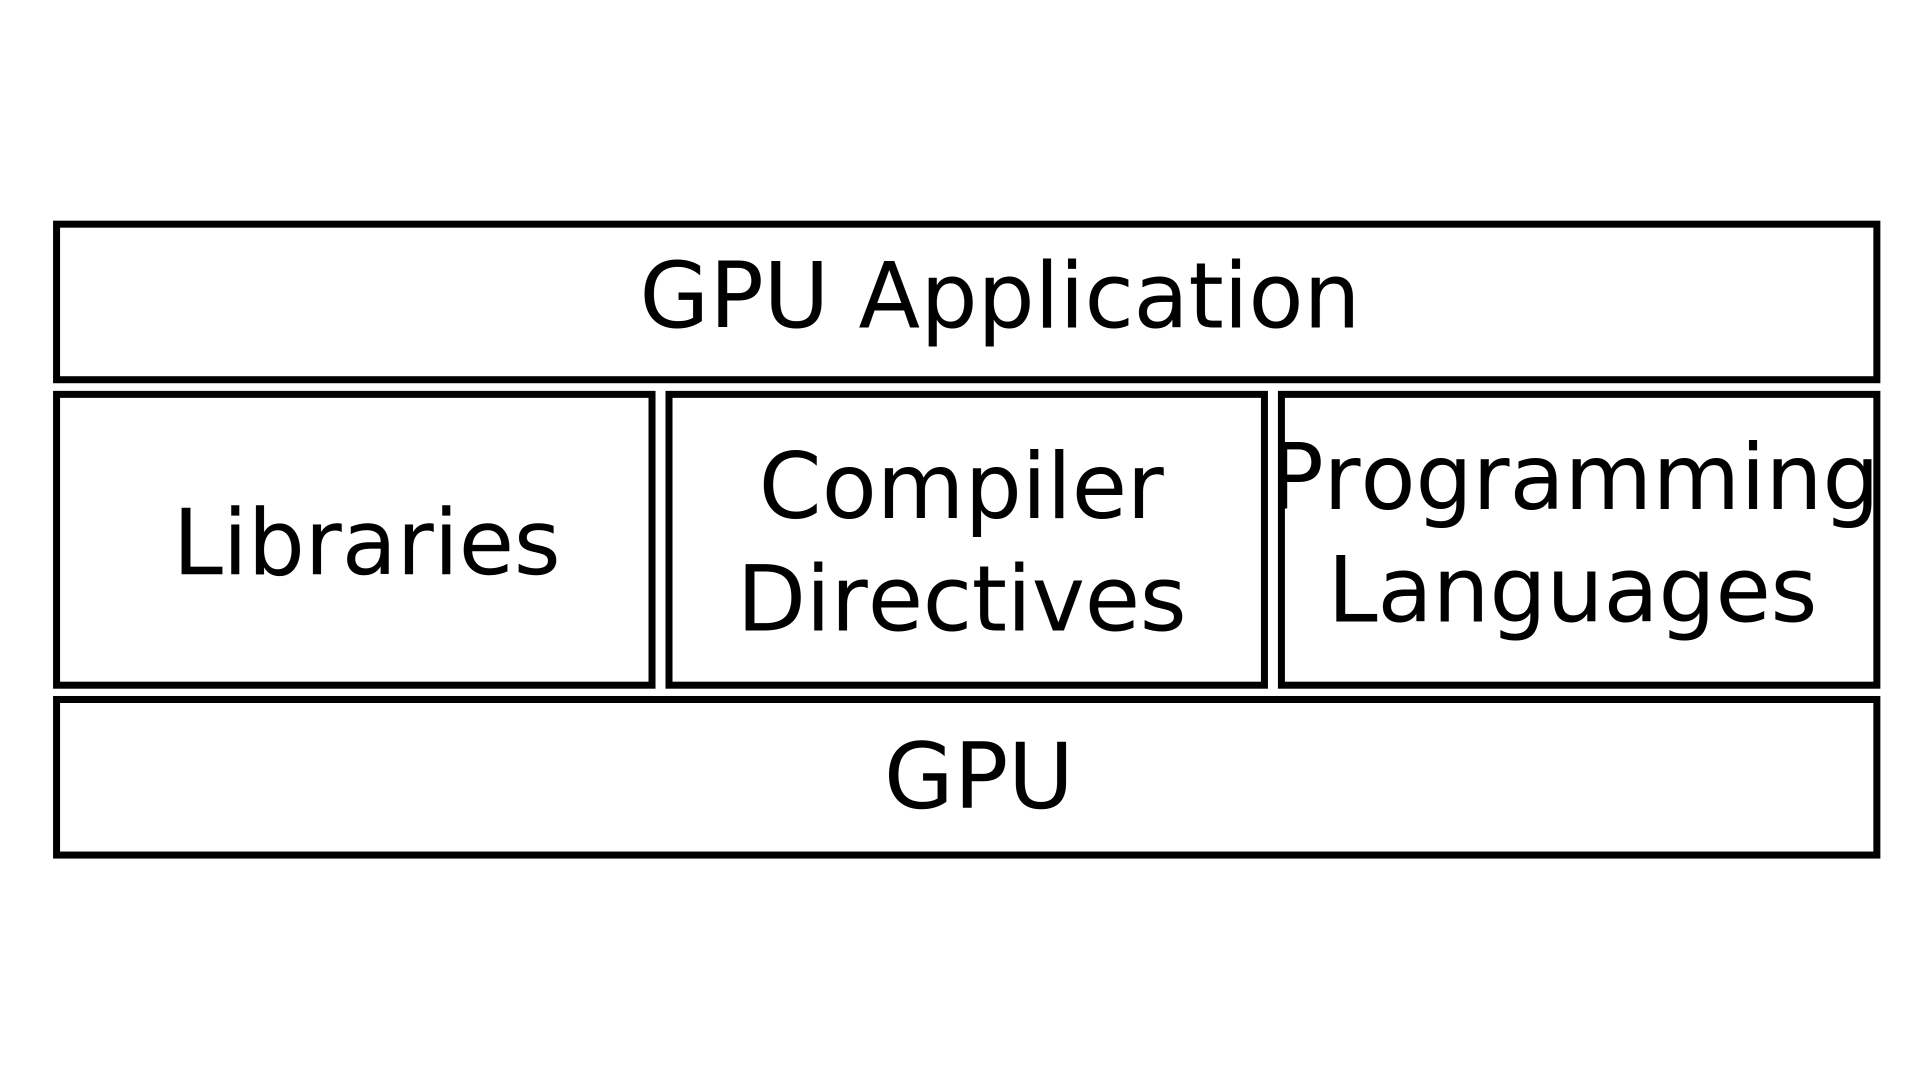
\includegraphics[width=.95\textwidth]{accel_apps}
\end{frame}

\subsection{Libraries}

\begin{frame}
    \frametitle{Libraries}
    \begin{center}
        \includegraphics[width=.6\textwidth]{accel_apps_lib}
    \end{center}
    \pause

    \begin{itemize}
        \item Easy to use
            \pause
        \item \alert{Drop-in} acceleration
            \pause
        \item Optimized by specialists
    \end{itemize}
\end{frame}

\begin{frame}
    \frametitle{Libraries}
    \centering
    \includegraphics[width=.9\textwidth]{accel_libs_no}
    \vfill

    \tiny{Image: \url{developer.nvidia.com/gpu-accelerated-libraries} [Accessed in 29/07/16]}
\end{frame}

\begin{frame}[fragile]
    \frametitle{Libraries}
    Vector sum with the \alert{Thrust} library:
    \begin{lstlisting}
    thrust::device_vector<float> device_input1(input_lenght);
    thrust::device_vector<float> device_input2(input_lenght);
    thrust::device_vector<float> device_output(input_lenght);
    \end{lstlisting}
    \pause
    \begin{lstlisting}
    thrust::copy(host_input1, host_input1 + input_lenght, device_input1.begin());

    thrust::copy(host_input2, host_input2 + input_lenght, device_input2.begin());
    \end{lstlisting}
    \pause
    \begin{lstlisting}
    thrust::transform(device_input1.begin(), device_input1.end(), device_input2.begin(), device_output.begin(), thrust::plus<float>());
    \end{lstlisting}
\end{frame}

\subsection{Compiler Directives}

\begin{frame}
    \frametitle{Compiler Directives}
    \begin{center}
        \includegraphics[width=.6\textwidth]{accel_apps_comp}
    \end{center}
    \pause

    \begin{itemize}
        \item Easy to use
            \pause
        \item Portable, but performance depends on compiler
    \end{itemize}
\end{frame}

\begin{frame}[fragile]
    \frametitle{Compiler Directives}
    Vector sum with \alert{OpenACC}:
    \begin{lstlisting}
    #pragma acc data copyin(input1[0:input_lenght],input2[0:input_lenght]), copyout(output[0:input_lenght])
    \end{lstlisting}
    \pause
    \begin{lstlisting}
    {
        #pragma acc kernels loop independent
        for(i = 0; i < input_lenght; i++) {
            output[i] = input1[i] + input2[i];
        }
    }
    \end{lstlisting}
\end{frame}

\subsection{Programming Languages}

\begin{frame}
    \frametitle{Programming Languages}
    \begin{center}
        \includegraphics[width=.6\textwidth]{accel_apps_lang}
    \end{center}
    \pause

    \begin{itemize}
        \item Best performance, but hard to master
            \pause
        \item Flexible
    \end{itemize}
\end{frame}

\begin{frame}
    \frametitle{Programming Languages}
    CUDA implementations in:
    \begin{itemize}
        \item \alert{C/C++}
        \item Fortran
        \item Python
        \item F\#
    \end{itemize}
\end{frame}

\section{CUDA C}

\begin{frame}
    \frametitle{CUDA C}
    \begin{center}
        \includegraphics[width=.3\textwidth]{cuda-c}
    \end{center}

    \pause
    Programming Model:
    \pause
    \begin{itemize}
        \item \alert{Kernels}
            \pause
        \item \alert{Threads} hierarchy
            \pause
        \item \alert{Memory} hierarchy
            \pause
        \item \alert{Heterogeneous} Programming
    \end{itemize}
\end{frame}

\subsection{Kernel}

\begin{frame}
    \frametitle{CUDA C: Kernel}
    \alert{Kernels}:
    \begin{itemize}
        \item \alert{Kernels} are C functions executed by \alert{threads}
        \item $N$ \textit{threads} run $N$ \textit{kernels}
            \pause
        \item Access thread \alert{ID}s using the \alert{\texttt{threadIdx}} variable
            \pause
        \item Defined within the \alert{\texttt{\_\_global\_\_}} scope
        \item Its type must be \alert{\texttt{void}}
    \end{itemize}

    \vfill

    \begin{center}
        \tiny{Source: \url{docs.nvidia.com/cuda/cuda-c-programming-guide/index.html\#programming-model} [Accessed in 29/07/16]}
    \end{center}
\end{frame}

\begin{frame}
    \frametitle{CUDA C: Kernel}
    \alert{Kernels}:
    \begin{itemize}
        \item Configured and launched using the syntax:
            \begin{itemize}
                \item \texttt{kernel\_name\alert{<<<}...\alert{>>>}(...);}
            \end{itemize}
            \pause
        \item Ideally executed in \alert{parallel}
            \pause
        \item In practice, parallelism depends on:
            \begin{itemize}
                \item Number of threads in a warp
                    \pause
                \item Execution branch coherence
            \end{itemize}
    \end{itemize}

    \vfill

    \begin{center}
        \tiny{Source: \url{docs.nvidia.com/cuda/cuda-c-programming-guide/index.html\#programming-model} [Accessed in 29/07/16]}
    \end{center}
\end{frame}

\begin{frame}[fragile]
    \frametitle{CUDA C: Kernel}
    Writing and \alert{launching} a \alert{kernel}:
    \begin{lstlisting}
    #include <cuda_runtime.h>

    __global__ void VecAdd(float* A, float* B, float* C) {
        int i = threadIdx.x;
        C[i] = A[i] + B[i];
    }
    \end{lstlisting}
    \pause
    \begin{lstlisting}
    int main() {
        ...
        VecAdd<<<1, N>>>(A, B, C);
        ...
    }
    \end{lstlisting}
    \vfill

    \begin{center}
        \tiny{Source: \url{docs.nvidia.com/cuda/cuda-c-programming-guide/index.html\#programming-model} [Accessed in 29/07/16]}
    \end{center}
\end{frame}

\subsection{Thread Hierarchy}

\begin{frame}
    \frametitle{CUDA C: Thread Hierarchy}
    \alert{Thread Block}:
    \begin{itemize}
        \item Grouping of threads
            \pause
        \item \alert{Tridimensional}: \texttt{\footnotesize{Db = (Dx, Dy, Dz)}}
            \pause
        \item \alert{Maximum size} of $1024$ threads
            \pause
        \item A \alert{Grid} is the tridimensional grouping of \textit{blocks}
    \end{itemize}

    \vfill

    \begin{center}
        \tiny{Source: \url{docs.nvidia.com/cuda/cuda-c-programming-guide/index.html\#programming-model} [Accessed in 29/07/16]}
    \end{center}
\end{frame}

\begin{frame}
    \frametitle{CUDA C: Thread Hierarchy}
    \centering
    \includegraphics[width=.7\textwidth]{grid-of-thread-blocks}

    \tiny{Source: \url{docs.nvidia.com/cuda/cuda-c-programming-guide/index.html\#programming-model} [Accessed in 29/07/16]}
\end{frame}

\begin{frame}
    \frametitle{Remembering: Pascal GP100 SM}
    \centering
    \includegraphics[width=.9\textwidth]{gp100_SM_diagram}

    \vfill

    \tiny{Image: \url{images.nvidia.com/content/pdf/tesla/whitepaper/pascal-architecture-whitepaper.pdf} [Accessed in 29/07/16]}
\end{frame}

\begin{frame}[fragile]
    \frametitle{CUDA C: Thread Hierarchy}
    \begin{lstlisting}
    __global__ void MatAdd(float A[N][N], float B[N][N], float C[N][N]) {
        int i = threadIdx.x;
        int j = threadIdx.y;
        C[i][j] = A[i][j] + B[i][j];
    }
    \end{lstlisting}
    \pause
    \begin{lstlisting}
    int main() {
        ...
        int numBlocks = 1;
        dim3 threadsPerBlock(N, N);
        MatAdd<<<numBlocks, threadsPerBlock>>>(A, B, C);
        ...
    }
    \end{lstlisting}
    \vfill

    \begin{center}
        \tiny{Source: \url{docs.nvidia.com/cuda/cuda-c-programming-guide/index.html\#programming-model} [Accessed in 29/07/16]}
    \end{center}
\end{frame}

\begin{frame}[fragile]
    \frametitle{CUDA C: Thread Hierarchy}
    \begin{lstlisting}
    __global__ void MatAdd(float A[N][N], float B[N][N], float C[N][N]) {
        int i = blockIdx.x * blockDim.x + threadIdx.x;
        int j = blockIdx.y * blockDim.y + threadIdx.y;
        if (i < N && j < N) {
            C[i][j] = A[i][j] + B[i][j];
        }
    }
    \end{lstlisting}
    \pause
    \begin{lstlisting}
    int main() {
        ...
        dim3 threadsPerBlock(16, 16);
        dim3 numBlocks(N / threadsPerBlock.x, N / threadsPerBlock.y);
        MatAdd<<<numBlocks, threadsPerBlock>>>(A, B, C);
        ...
    }
    \end{lstlisting}
    \vfill

    \begin{center}
        \tiny{Source: \url{docs.nvidia.com/cuda/cuda-c-programming-guide/index.html\#programming-model} [Accessed in 29/07/16]}
    \end{center}
\end{frame}

\begin{frame}[fragile]
    \frametitle{CUDA C: Thread Hierarchy}
    Configuration and Launching syntax \texttt{\scriptsize{\alert{<<<} Dg, Db, Ns, S \alert{>>>}}}:
    \begin{itemize}
        \item \texttt{\alert{dim3} Dg} grid dimension and size:
\begin{lstlisting}
Dg.x * Dg.y * Dg.z = numBlocks
\end{lstlisting}
        \pause
        \item \texttt{\alert{dim3} Db} block dimension and size:
\begin{lstlisting}
Db.x * Db.y * Db.z = threadsPerBlock
\end{lstlisting}
        \pause
        \item \texttt{\alert{size\_t} Ns = 0}: extra bytes in shared memory
        \item \texttt{\alert{cudaStream\_t} S = 0}: CUDA stream
    \end{itemize}

    \vfill

    \begin{center}
        \tiny{Source: \url{docs.nvidia.com/cuda/cuda-c-programming-guide/index.html\#programming-model} [Accessed in 29/07/16]}
    \end{center}
\end{frame}

\subsection{Memory Hierarchy}

\begin{frame}
    \frametitle{CUDA C: Memory Hierarchy}
    Threads access \alert{multiple memory addresses} during a kernel's execution:
    \begin{itemize}
        \item Local
            \pause
        \item Shared with its \textit{block}
            \pause
        \item Global\pause: persists between kernels of the \alert{same application}
            \pause
        \item \textit{Read-only}
    \end{itemize}
    \vfill

    \begin{center}
        \tiny{Source: \url{docs.nvidia.com/cuda/cuda-c-programming-guide/index.html\#programming-model} [Accessed in 29/07/16]}
    \end{center}
\end{frame}

\begin{frame}
    \frametitle{CUDA C: Memory Hierarchy}
    \begin{center}
        \includegraphics[width=.5\textwidth]{cuda-memory-hierarchy}
    \end{center}

    \vfill

    \begin{center}
        \tiny{Source: \url{docs.nvidia.com/cuda/cuda-c-programming-guide/index.html\#programming-model} [Accessed in 29/07/16]}
    \end{center}
\end{frame}

\subsection{Heterogeneous Programming}

\begin{frame}
    \frametitle{CUDA C: Heterogeneous Programming}
    \alert{Host}'s tasks:
    \begin{itemize}
        \item Allocate \alert{device} memory and resources
        \item Move \alert{data} (\alert{bottleneck!})
            \pause
        \item Launch kernel
            \pause
        \item Move \alert{results} (\alert{bottleneck!})
        \item Release \alert{device} memory and resources
    \end{itemize}
    \pause
    \alert{Device}'s tasks:
    \begin{itemize}
        \item Run kernel
    \end{itemize}
\end{frame}

\begin{frame}
    \frametitle{CUDA C: Heterogeneous Programming}
    \centering
    \includegraphics[width=.8\textwidth]{accel}
\end{frame}

\subsection{Example: Vector Sum}

\begin{frame}[fragile]
    \frametitle{Example: Vector Sum}
    \begin{lstlisting}
    __global__ void vectorAdd(const float *A, const float *B, float *C, int numElements) {
        int i = blockDim.x * blockIdx.x + threadIdx.x;

        if (i < numElements) {
            C[i] = A[i] + B[i];
        }
    }
    \end{lstlisting}

    \vfill

    \begin{center}
        \tiny{Source: \url{github.com/phrb/intro-cuda} [Accessed in 29/07/16]}
    \end{center}
\end{frame}

\begin{frame}[fragile]
    \frametitle{Example: Vector Sum}
    \begin{lstlisting}[basicstyle=\ttfamily\scriptsize]
    #include <cuda_runtime.h>
    \end{lstlisting}
    \pause
    \begin{lstlisting}[basicstyle=\ttfamily\scriptsize]
    float *h_A = (float *) malloc(size);
    if (h_A == NULL) { ... };

    float *d_A = NULL;
    err = cudaMalloc((void **) &d_A, size);
    err = cudaMemcpy(d_A, h_A, size, cudaMemcpyHostToDevice);
    if (err != cudaSuccess) { ... };
    \end{lstlisting}
    \pause
    \begin{lstlisting}[basicstyle=\ttfamily\scriptsize]
    int threadsPerBlock = 256;
    int blocksPerGrid = (numElements + threadsPerBlock - 1) / threadsPerBlock;
    \end{lstlisting}
    \pause
    \begin{lstlisting}[basicstyle=\ttfamily\scriptsize]
    vectorAdd<<<blocksPerGrid, threadsPerBlock>>>(d_A, d_B, d_C, numElements);

    err = cudaGetLastError()
    err = cudaDeviceSynchronize()
    if (err != cudaSuccess) { ... };
    \end{lstlisting}
    \pause
    \begin{lstlisting}[basicstyle=\ttfamily\scriptsize]
    err = cudaMemcpy(h_C, d_C, size, cudaMemcpyDeviceToHost);
    err = cudaFree(d_A);
    if (err != cudaSuccess) { ... };
    \end{lstlisting}

    \vfill

    \begin{center}
        \tiny{Source: \url{github.com/phrb/intro-cuda} [Accessed in 29/07/16]}
    \end{center}
\end{frame}

\begin{frame}[fragile]
    \frametitle{Example: Practical Tip}
    \alert{Always} check for errors!

    \begin{lstlisting}
    float *d_A = NULL;
    err = cudaMalloc((void **) &d_A, size);

    err = cudaGetLastError()

    err = cudaDeviceSynchronize()
    \end{lstlisting}
    \pause
    \begin{lstlisting}
    if (err != cudaSuccess) {
        fprintf(stderr, "Failed to allocate device vector A (error code %s)!\n", cudaGetErrorString(err));
        exit(EXIT_FAILURE);
    }
    \end{lstlisting}

    \begin{center}
        \tiny{Source: \url{github.com/phrb/intro-cuda} [Accessed in 29/07/16]}
    \end{center}
\end{frame}

\subsection{Hands on!}

\begin{frame}
    \frametitle{Hands on!}
    We'll run some CUDA C samples available at
    \url{github.com/phrb/intro-cuda}:
    \begin{itemize}
        \item \url{src/cuda-samples/0_Simple/vectorAdd}
            \pause
        \item \url{src/cuda-samples/5_Simulations/fluidsGL}
        \item \url{src/cuda-samples/5_Simulations/oceanFFT}
        \item \url{src/cuda-samples/5_Simulations/smokeParticles}
            \pause
        \item \url{src/mandelbrot_numba}
    \end{itemize}
\end{frame}

\subsection{Resources}

\begin{frame}
    \frametitle{Resources}
    This presentation and all source code are available
    at \alert{GitHub}:

    \begin{itemize}
        \item \url{github.com/phrb/intro-cuda}
    \end{itemize}

    More resources:

    \begin{itemize}
        \item CUDA C: \url{docs.nvidia.com/cuda/cuda-c-programming-guide}
        \item CUDA Toolkit: \url{developer.nvidia.com/cuda-toolkit}
        \item Best Practices Guide:
            \begin{itemize}
                \item \url{docs.nvidia.com/cuda/cuda-c-best-practices-guide}
            \end{itemize}
        \item GPU Teaching Kit: \url{syllabus.gputeachingkit.com}
        \item iPython: \url{ipython.org/notebook.html}
        \item Anaconda: \url{continuum.io/downloads}
    \end{itemize}
\end{frame}

\part{Part II}

\maketitle

\section{Recapitulation}

\subsection{About}

\begin{frame}
    \frametitle{About}
    \footnotesize
    \begin{columns}[T,onlytextwidth]
        \column{0.5\textwidth}
        \begin{center}
            \includegraphics[width=.42\textwidth]{pedro}

            Pedro Bruel

            \alert{phrb}@ime.usp.br
        \end{center}

        \column{0.5\textwidth}
        \begin{center}
            \includegraphics[width=.37\textwidth]{alfredo}

            Alfredo Goldman

            \alert{gold}@ime.usp.br
        \end{center}

    \end{columns}

    \begin{center}
        \includegraphics[width=.18\textwidth]{gubi}

        Marco Dimas Gubitoso

        \alert{gubi}@ime.usp.br
    \end{center}
\end{frame}

\subsection{Summary}

\begin{frame}
    \frametitle{Part I}
    \setbeamertemplate{section in toc}[sections numbered]
    \tableofcontents[hideallsubsections, part=1]
\end{frame}

\begin{frame}
    \frametitle{Part II}
    \setbeamertemplate{section in toc}[sections numbered]
    \tableofcontents[hideallsubsections, part=2]
\end{frame}

\begin{frame}
    \frametitle{Slides}
    \begin{center}
        \includegraphics[width=.18\textwidth]{github}
    \end{center}
    This presentation and all source code are available
    at \alert{GitHub}:

    \begin{itemize}
        \item \url{github.com/phrb/intro-cuda}
    \end{itemize}
\end{frame}

\subsection{Recapitulating}

\begin{frame}
    \frametitle{Hardware Acceleration}
    \begin{center}
        \includegraphics[width=.6\textwidth]{accelerate}
    \end{center}

    The use of \alert{devices} to accelerate computations on large datasets:

    \begin{itemize}
        \item Associated with a \alert{host} processor
        \item Separate \alert{control} and \alert{memory}
        \item Differ on \alert{specialization} and \alert{configurability}
        \item \alert{GPUs}, DSPs, FPGAs, ASICs
    \end{itemize}
\end{frame}

\begin{frame}
    \frametitle{Hardware Acceleration}
    \centering
    \includegraphics[width=.8\textwidth]{accel}
\end{frame}

\begin{frame}
    \frametitle{Hardware Acceleration}
    Percentage of systems with accelerators in the \textit{Top500}:

    \begin{center}
    \includegraphics[width=.95\textwidth]{top500_accel}
    \hfill

        \tiny{Image: \url{top500.org/lists/2016/06/download/TOP500_201606_Poster.pdf} [Accessed in 29/07/16]}
    \end{center}
\end{frame}

\subsection{Heterogeneous Computing}

\begin{frame}
    \frametitle{Heterogeneous Computing}
    \begin{center}
        \includegraphics[width=.83\textwidth]{titan}
    \end{center}

    Given \alert{heterogeneous} computational resources, \alert{datasets}
    and a set of \alert{computations}, how to distribute data and computations
    to \alert{optimize resource usage}?
    \hfill

    \begin{center}
    \tiny{Image: \url{olcf.ornl.gov/titan} [Accessed in 29/07/16]}
    \end{center}
\end{frame}

\begin{frame}
    \frametitle{Graphics Processing Units}
    \begin{center}
        \includegraphics[width=.6\textwidth]{gtx1080}
    \end{center}
    \pause

    Originally specialized for \alert{graphical processing},
    optimized for large datasets and \alert{high throughput}:

    \begin{itemize}
        \item Small caches (\textit{kilobytes})
        \item No \alert{branch prediction}
        \item Thousands of \alert{higher latency} ALUs
        \item Execution \alert{pipelines}
        \item 114 688 concurrent \alert{threads} in Pascal architecture
    \end{itemize}
\end{frame}

\begin{frame}
    \frametitle{CUDA Platform}
    \begin{center}
        \includegraphics[width=.4\textwidth]{cuda-logo}
    \end{center}

    \begin{itemize}
        \item A platform for \alert{parallel computing}
        \item \textit{Application Programming Interface} (API)
        \item CUDA \textit{Toolkit}
    \end{itemize}
\end{frame}

\begin{frame}
    \frametitle{Programming Languages}
    \begin{center}
        \includegraphics[width=.6\textwidth]{accel_apps_lang}
    \end{center}

    \begin{itemize}
        \item Best performance, but hard to master
        \item Flexible
    \end{itemize}
\end{frame}

\begin{frame}
    \frametitle{CUDA C}
    \begin{center}
        \includegraphics[width=.3\textwidth]{cuda-c}
    \end{center}

    Programming Model:

    \begin{itemize}
        \item \alert{Kernels}
        \item \alert{Threads} hierarchy
        \item \alert{Memory} hierarchy
        \item \alert{Heterogeneous} Programming
    \end{itemize}
\end{frame}

\begin{frame}[fragile]
    \frametitle{Example: Vector Sum}
    \begin{lstlisting}[basicstyle=\ttfamily\scriptsize]
    #include <cuda_runtime.h>

    float *h_A = (float *) malloc(size);
    if (h_A == NULL) { ... };

    float *d_A = NULL;
    err = cudaMalloc((void **) &d_A, size);
    err = cudaMemcpy(d_A, h_A, size, cudaMemcpyHostToDevice);
    if (err != cudaSuccess) { ... };

    int threadsPerBlock = 256;
    int blocksPerGrid = (numElements + threadsPerBlock - 1) / threadsPerBlock;

    vectorAdd<<<blocksPerGrid, threadsPerBlock>>>(d_A, d_B, d_C, numElements);

    err = cudaGetLastError()
    err = cudaDeviceSynchronize()
    if (err != cudaSuccess) { ... };

    err = cudaMemcpy(h_C, d_C, size, cudaMemcpyDeviceToHost);
    err = cudaFree(d_A);
    if (err != cudaSuccess) { ... };
    \end{lstlisting}

    \vfill

    \begin{center}
        \tiny{Source: \url{github.com/phrb/intro-cuda} [Accessed in 29/07/16]}
    \end{center}
\end{frame}

\begin{frame}
    \frametitle{Hands on!}
    We'll run some CUDA C samples available at
    \url{github.com/phrb/intro-cuda}:
    \begin{itemize}
        \item \url{src/cuda-samples/0_Simple/vectorAdd}
        \item \url{src/cuda-samples/5_Simulations/fluidsGL}
        \item \url{src/cuda-samples/5_Simulations/oceanFFT}
        \item \url{src/cuda-samples/5_Simulations/smokeParticles}
        \item \url{src/mandelbrot_numba}
    \end{itemize}
\end{frame}

\begin{frame}[fragile]
    \frametitle{Example: Practical Tip}
    \alert{Always} check for errors!

    \begin{lstlisting}
    float *d_A = NULL;
    err = cudaMalloc((void **) &d_A, size);

    err = cudaGetLastError()

    err = cudaDeviceSynchronize()

    if (err != cudaSuccess) {
        fprintf(stderr, "Failed to allocate device vector A (error code %s)!\n", cudaGetErrorString(err));
        exit(EXIT_FAILURE);
    }
    \end{lstlisting}

    \begin{center}
        \tiny{Source: \url{github.com/phrb/intro-cuda} [Accessed in 29/07/16]}
    \end{center}
\end{frame}

\section{Compiling CUDA Applications}

\subsection{NVIDIA CUDA Compiler}

\begin{frame}
    \frametitle{Nvidia CUDA Compiler (\texttt{nvcc})}
    \begin{center}
        \includegraphics[width=.55\textwidth]{compiler}
    \end{center}
    \pause
    \begin{itemize}
        \item \alert{Proprietary} system
            \pause
        \item Uses the host's C++ compiler
            \pause
        \item Compiles CUDA code to \textit{Parallel Thread Execution} (\alert{PTX} ISA)
            \pause
        \item Host's code + Device's code $\rightarrow$ \alert{fatbinary}
    \end{itemize}
\end{frame}

\subsection{Programming Model}

\begin{frame}
    \frametitle{\texttt{nvcc}: CUDA programming model}
    \begin{itemize}
        \item SIMD, SIMT
        \item \textit{Single Program Multiple Data} (SPMD)
            \pause
        \item Device: \alert{parallel} and \alert{independent} threads
        \item \textit{Host}: does not interfere
    \end{itemize}
\end{frame}

\subsection{Compilation Trajectory}

\begin{frame}
    \frametitle{\texttt{nvcc}: Compilation Trajectory}
    \centering
    \includegraphics[width=.7\textwidth]{cuda-compilation}
    \vfill

    \begin{center}
        \tiny{Image: \url{docs.nvidia.com/cuda/cuda-compiler-driver-nvcc} [Accessed in 29/07/16]}
    \end{center}
\end{frame}

\section{Optimization Best Practices}

\subsection{Measure, Parallelize, Optimize, Deploy}

\begin{frame}
    \frametitle{Measure, Parallelize, Optimize, Deploy}
    \centering
    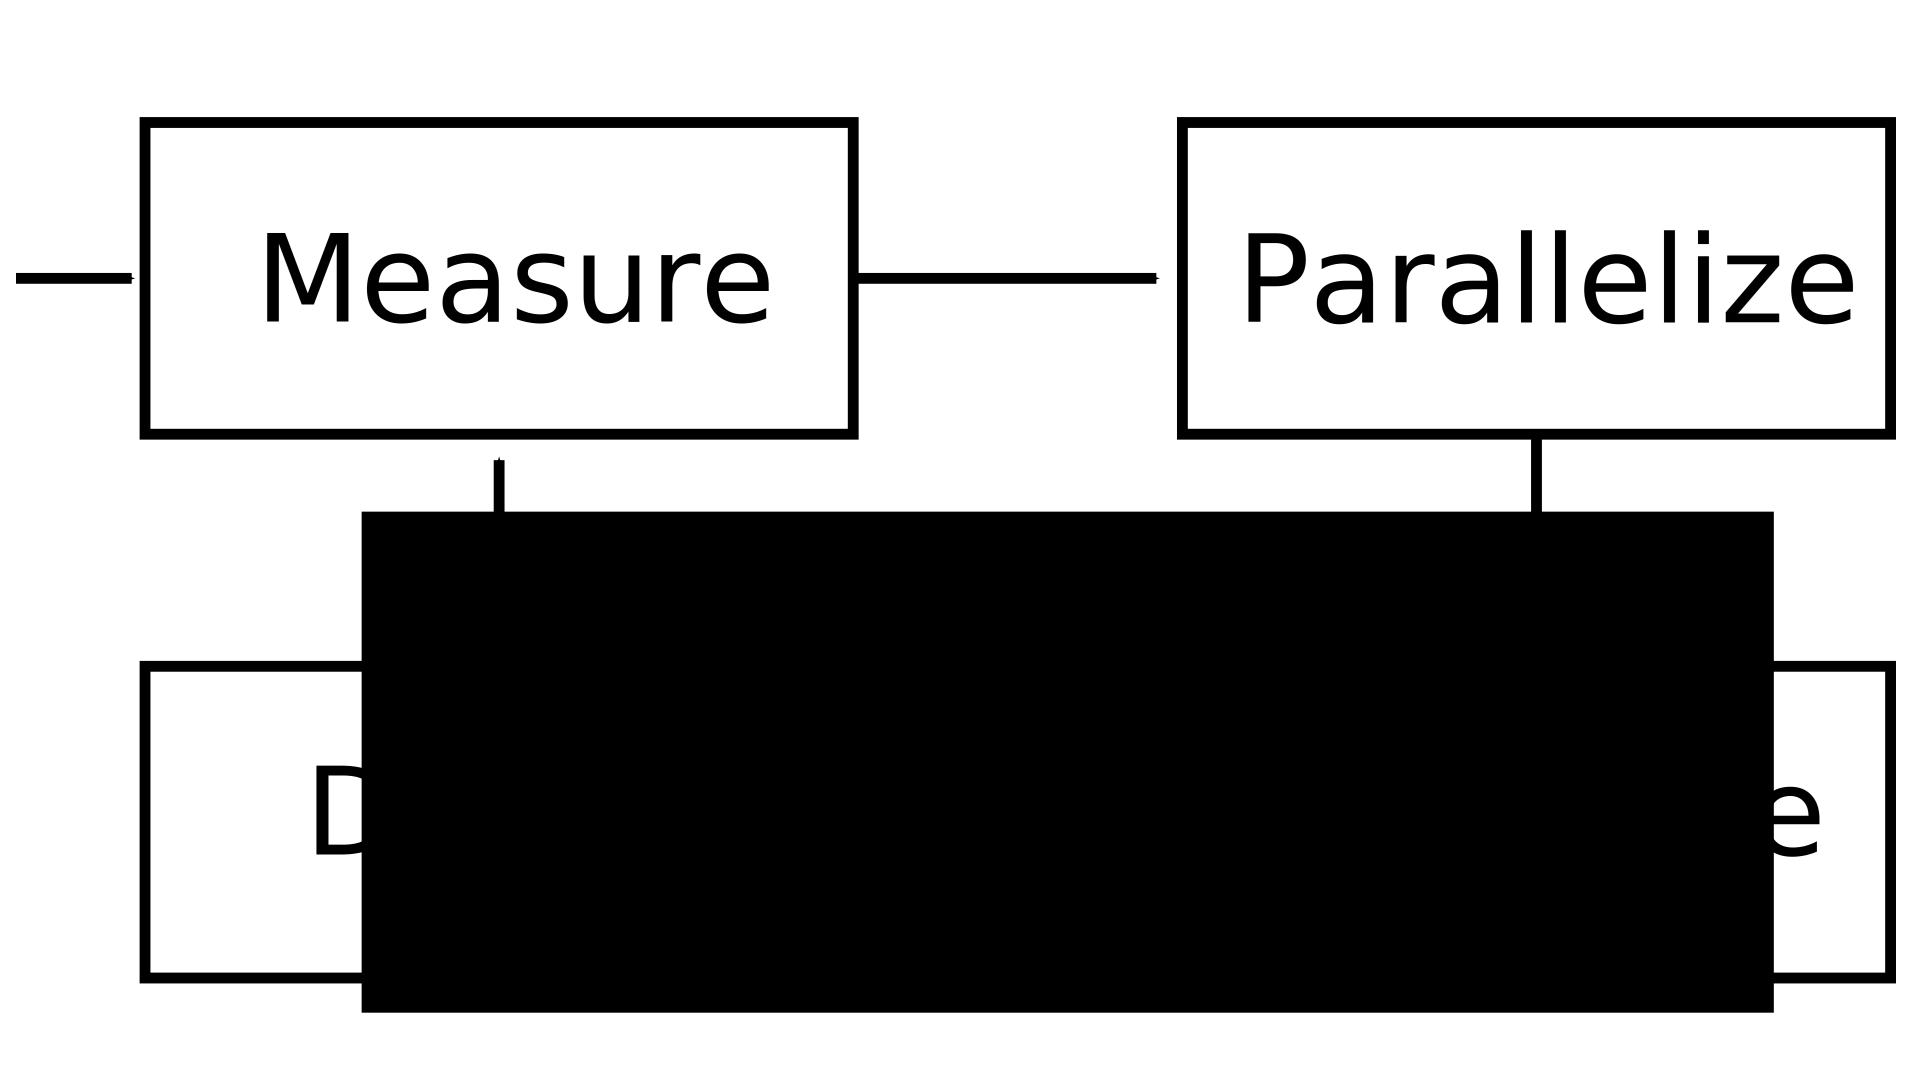
\includegraphics[width=.9\textwidth]{MPOD}
    \vfill

    \begin{center}
        \tiny{Source: \url{docs.nvidia.com/cuda/cuda-c-best-practices-guide} [Accessed in 29/07/16]}
    \end{center}
\end{frame}

\subsection{Measure}

\begin{frame}
    \frametitle{Measure}
    \begin{center}
    \includegraphics[width=.4\textwidth]{MPOD_M}
    \end{center}
    \vfill

    \pause
    Given a \alert{sequential program}:
    \begin{itemize}
        \item Which functions do the \alert{heavy lifting} (\alert{bottlenecks})?
            \pause
        \item Can they be \alert{parallelized}?
            \pause
        \item How does your program behaves when:
            \begin{itemize}
                \item The work is divided between more processes? (\alert{strong scaling})
                    \pause
                \item There is more work to be done? (\alert{weak scaling})
            \end{itemize}
    \end{itemize}
\end{frame}

\subsection{Parallelize}

\begin{frame}
    \frametitle{Parallelize}
    \begin{center}
    \includegraphics[width=.4\textwidth]{MPOD_P}
    \vfill
        \pause
    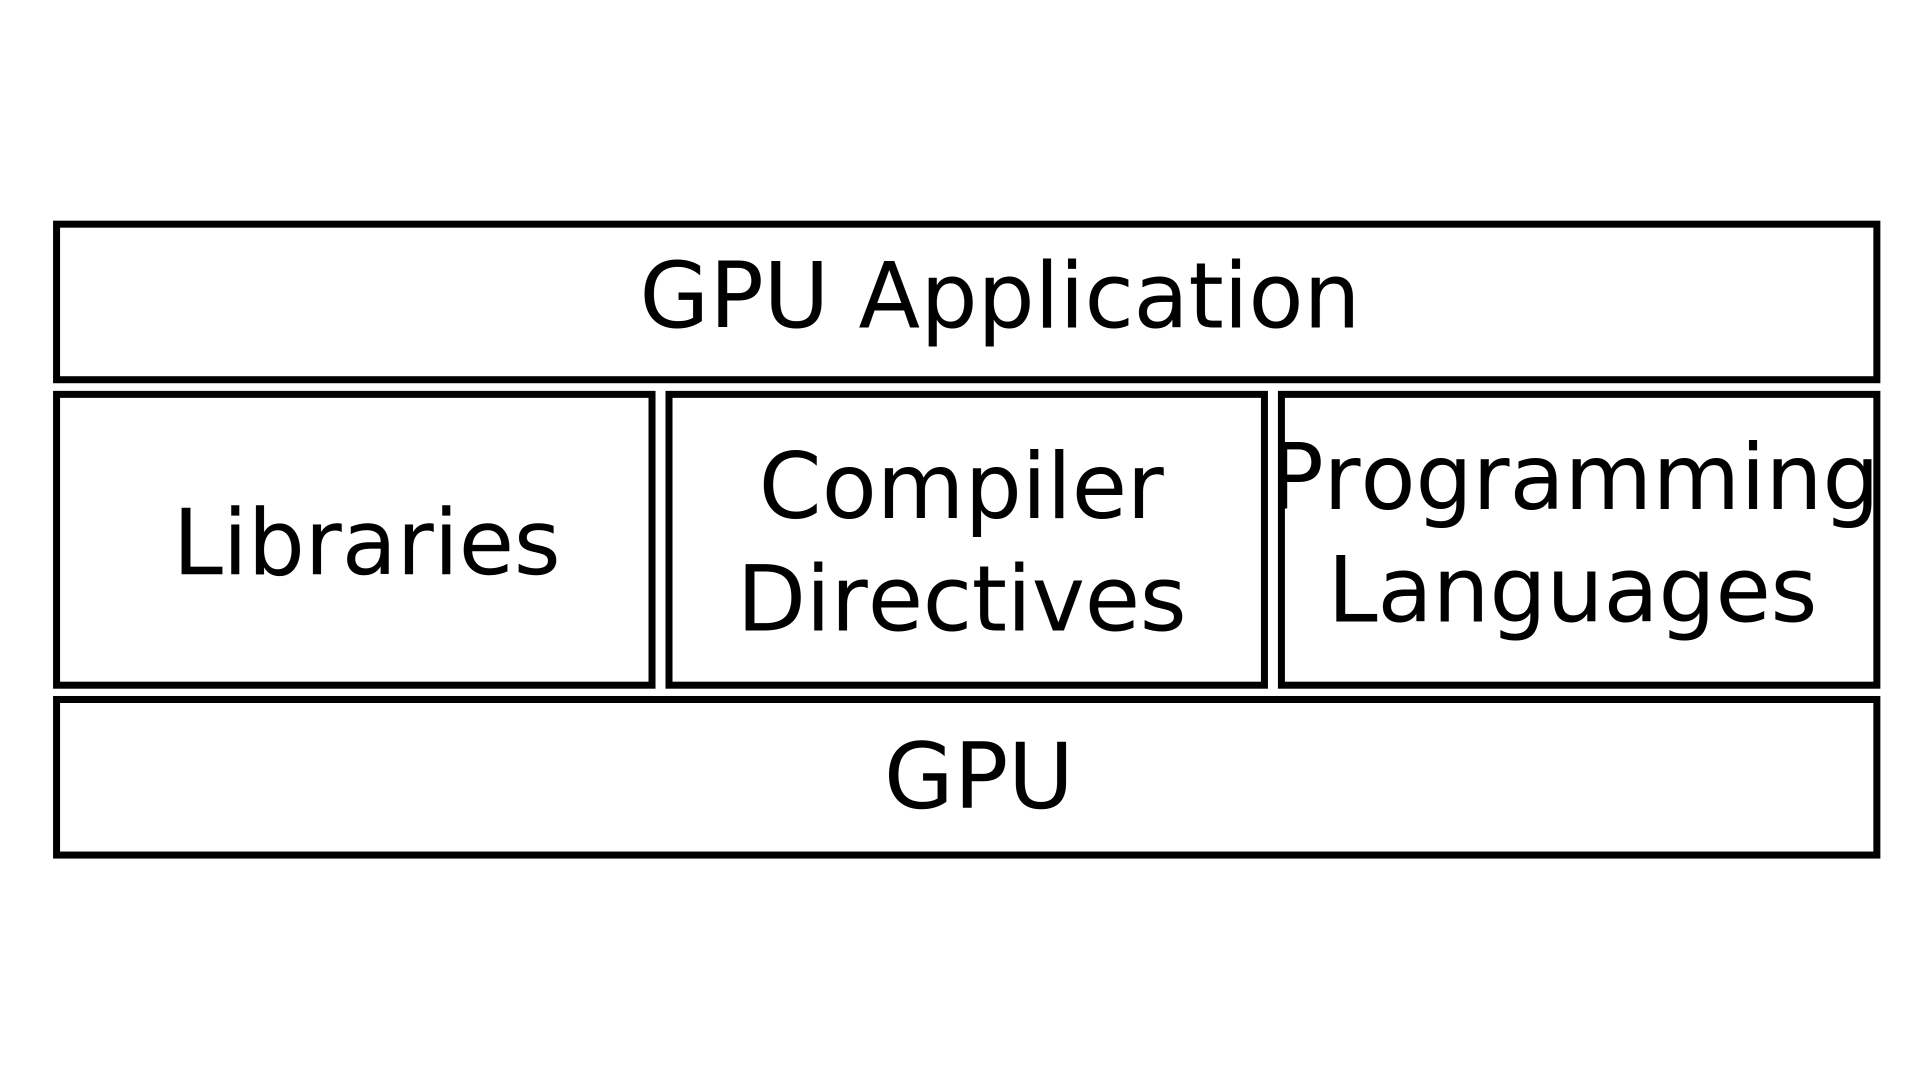
\includegraphics[width=.6\textwidth]{accel_apps}
    \end{center}
\end{frame}

\begin{frame}
    \frametitle{Parallelize}
    \begin{center}
    \includegraphics[width=.4\textwidth]{MPOD_P}
    \vfill
    \includegraphics[width=.5\textwidth]{accel_libs_no}
    \end{center}
\end{frame}

\subsection{Optimze}

\begin{frame}
    \frametitle{Optimize}
    \begin{center}
    \includegraphics[width=.4\textwidth]{MPOD_O}
    \end{center}

    \vfill

    \pause
    Optimization:
    \begin{itemize}
        \item \alert{Cyclical} \pause and \alert{incremental}
            \pause
        \item Applicable to \alert{different levels}
            \pause
        \item \alert{Tools} are very important
    \end{itemize}

    \pause
    \begin{center}
    \alert{Efficiency} with algorithms, \pause \alert{performance} with data structures
    \end{center}
\end{frame}

\subsection{Deploy}

\begin{frame}
    \frametitle{Deploy}
    \begin{center}
    \includegraphics[width=.4\textwidth]{MPOD_D}
    \end{center}

    \vfill

    \pause
    \begin{itemize}
        \item Prepare application for \alert{measurement}
            \pause
        \item \alert{Incremental} optimizations and changes
            \pause
        \item How much is it still \alert{possible} to optimize?
    \end{itemize}
\end{frame}

\section{Analysing CUDA Applications}

\begin{frame}
    \frametitle{Analysing CUDA Applications}
    \begin{center}
        \includegraphics[width=.2\textwidth]{data_profile}
    \end{center}

    \alert{Parallel} and \alert{distributed} computing is
    increasingly important, but \alert{legacy code} is often:
    \pause
    \begin{itemize}
        \item \alert{Sequential}
            \pause
        \item \alert{Coarse grained}
    \end{itemize}
    \pause

    Analysis or \alert{profiling}:
    \pause
    \begin{itemize}
        \item What are the \alert{hotspots} (\textit{bottlenecks})?
            \pause
        \item Can they be parallelized?
            \pause
        \item What are the relevant \alert{workloads}?
    \end{itemize}
\end{frame}

\subsection{Host and Device}

\begin{frame}
    \frametitle{Host and Device}
    Differences between host and device:
    \begin{itemize}
        \item Threading model
            \pause
        \item Memory
    \end{itemize}

    \pause
    What to run on \alert{GPUs}?
    \pause
    \begin{itemize}
        \item Large \alert{datasets}
            \pause
        \item \alert{Independent} computations
    \end{itemize}
    \pause

    Always consider the impact of \alert{data transferences}!
\end{frame}

\subsection{Profiling}

\begin{frame}
    \frametitle{\textit{Profiling}}
    Monitoring code during \alert{runtime}
    obtaining information for \alert{optimization}
    \pause

    Code \alert{instrumentation}:
    \begin{itemize}
        \item Capture \alert{events}
            \pause
        \item Generate \alert{data}
            \pause
        \item Tools
    \end{itemize}
\end{frame}

\begin{frame}
    \frametitle{\textit{Profiling: Flamegraphs}}
    \begin{center}
        \includegraphics[width=\textwidth]{flamegraph}
    \end{center}

    Help analyse:
    \begin{itemize}
        \item Performance \textit{bottlenecks}, \textit{hotspots}
            \pause
        \item Frequency and duration of \alert{function calls}: \textit{On-CPU}
            \pause
        \item \alert{Idle} time (\textit{waiting}): \textit{Off-CPU}
    \end{itemize}
\end{frame}

\begin{frame}
    \frametitle{Profiling: \texttt{nvprof}}
    A \alert{command line} profiler
    that enables collecting CUDA-related events:
    \pause
    \begin{itemize}
        \item CPU and GPU
            \pause
        \item Kernel execution
            \pause
        \item Memory usage and transferences
            \pause
        \item CUDA API
    \end{itemize}
    \pause

    Generates data for \alert{posterior visualization}

    \begin{center}
        \tiny{Source: \url{docs.nvidia.com/cuda/profiler-users-guide} [Accessed in 29/07/16]}
    \end{center}
\end{frame}

\begin{frame}
    \frametitle{Profiling: \texttt{nvvp}}
    \centering
    \includegraphics[width=\textwidth]{nvvp}

    \vfill
    \tiny{Source: \url{docs.nvidia.com/cuda/profiler-users-guide} [Accessed in 29/07/16]}
\end{frame}

\begin{frame}
    \frametitle{Profiling: Tools}
    \centering
    \includegraphics[width=.5\textwidth]{profile_tools}

    \vfill
    \tiny{Source: \url{developer.nvidia.com/performance-analysis-tools} [Accessed in 29/07/16]}
\end{frame}

\subsection{Debugging}

\begin{frame}
    \frametitle{\textit{Debugging}}
    Monitoring code during \alert{runtime}
    obtaining information for \alert{error correction} (\alert{bugs})
    \pause

    Code \alert{instrumentation}:
    \begin{itemize}
        \item \alert{Step-by-step} execution
            \pause
        \item \alert{Breakpoints}
            \pause
        \item Different \alert{threads}
            \pause
        \item CUDA \texttt{\alert{gdb}} and \texttt{\alert{memcheck}}
    \end{itemize}
    \pause

    Help fixing:
    \begin{itemize}
        \item Memory \alert{leaks}
            \pause
        \item \alert{Control flow} problems
            \pause
        \item ...
    \end{itemize}
\end{frame}

\section{Otimizing CUDA Applications}

\begin{frame}
    \frametitle{Optimizing CUDA Applications}
    \begin{center}
        \includegraphics[width=.2\textwidth]{optimization_icon}
    \end{center}

    Different \alert{abstraction} and \alert{priority} levels:
    \pause
    \begin{itemize}
        \item Memory
            \pause
        \item Control flow
            \pause
        \item Execution configuration
            \pause
        \item Instruction selection
    \end{itemize}
\end{frame}

\subsection{Memory Optimizations}

\begin{frame}
    \frametitle{Memory Optimizations}
    The \alert{most important} for \alert{high performance}
    \pause

    Objectives:
    \begin{itemize}
        \item Maximize \alert{bandwidth}
            \pause
        \item Minimize \alert{transferences} between device and host
            \pause
    \end{itemize}

    Best practices:
    \pause

    \begin{itemize}
        \item Device:
            \pause
            \begin{itemize}
                \item Prioritize \alert{computations}
                    \pause
                \item Create and destroy \alert{intermediate data structures}
                    \pause
                \item \alert{Grouped} (\textit{coalescent}) memory accesses
            \end{itemize}
            \pause
        \item Host:
            \pause
            \begin{itemize}
                \item Delegate \alert{computations}
                    \pause
                \item Minimize \alert{data transferences}
            \end{itemize}
    \end{itemize}
\end{frame}

\subsection{Control Flow Optimizations}

\begin{frame}
    \frametitle{Control Flow Optimizations}
    \alert{High priority} for \alert{high performance}
    \pause

    Objectives:
    \begin{itemize}
        \item Avoid \alert{Control Flow divergence} inside warps
            \pause
        \item \texttt{\alert{if}}, \texttt{\alert{switch}},
            \texttt{\alert{do}}, \texttt{\alert{for}}, \texttt{\alert{while}}
            \pause
        \item Use \texttt{\alert{threadIdx}} efficiently
    \end{itemize}
\end{frame}

\subsection{Execution Configuration Optimizations}

\begin{frame}
    \frametitle{Execution Configuration Optimizations}
    How to use the \alert{device}'s potential?
    \pause
    \begin{itemize}
        \item Maximize \alert{occupancy}
            \pause
        \item Efficiently allocate \alert{blocks} and \alert{threads}
            \pause
        \item Independent \alert{kernel} executions
    \end{itemize}
\end{frame}

\subsection{Instruction Selection Optimizations}

\begin{frame}
    \frametitle{Instruction Selection Optimizations}
    \alert{Low priority} for \alert{high performance}:
    \pause
    \begin{itemize}
        \item \alert{Low level}
            \pause
        \item Applied to \alert{hotspots}
            \pause
        \item Applied by \alert{experts}
        \item Only after \alert{exhausting} other optimizations
    \end{itemize}
\end{frame}

\section{Conclusion}

\begin{frame}
    \frametitle{Conclusion}
    \centering
        \includegraphics[width=.75\textwidth]{top500_accel}
    \vfill

    Achieve \alert{high performance} using \alert{accelerators} \pause (\alert{GPUs})
\end{frame}

\begin{frame}
    \frametitle{Conclusion}
    \begin{center}
        \includegraphics[width=.5\textwidth]{titan_x}
    \end{center}
    \vfill

    \pause
    \alert{Implementation}, \alert{analysis} and \alert{optimization} costs

    \pause
    CUDA Platform \alert{tools}
\end{frame}

\subsection{Resources}

\begin{frame}
    \frametitle{Resources}
    This presentation and all source code are available
    at \alert{GitHub}:

    \begin{itemize}
        \item \url{github.com/phrb/intro-cuda}
    \end{itemize}

    More resources:

    \begin{itemize}
        \item CUDA C: \url{docs.nvidia.com/cuda/cuda-c-programming-guide}
        \item CUDA Toolkit: \url{developer.nvidia.com/cuda-toolkit}
        \item Best Practices Guide:
            \begin{itemize}
                \item \url{docs.nvidia.com/cuda/cuda-c-best-practices-guide}
            \end{itemize}
        \item GPU Teaching Kit: \url{syllabus.gputeachingkit.com}
        \item iPython: \url{ipython.org/notebook.html}
        \item Anaconda: \url{continuum.io/downloads}
    \end{itemize}
\end{frame}

\maketitle

\end{document}
